\chapter{Realisatie}
\label{ch:realization}

\section{Software}

De software van het Autonerf systeem is geïmplementeerd in C++ waarbij gebruikt
wordt gemaakt van de libraries van OpenCV. OpenCV is een groep libraries die
ontwikkeld zijn voor \emph{computer vision} (OpenCV staat dan ook voor
\emph{Open Computer Vision}).

De software is \emph{event driven} geschreven. Dit betekend dat, in plaats dat
er gepolled wordt door object voor data, er met events wordt gewerkt. Wanneer
er binnen een object een event plaatsvindt, worden andere \emph{subscribers}
hier van op de hoogte gebracht.

Events worden met een basisklasse (\code{Autonerf::Emitter}) ge-\emph{emit}.
Objecten kunnen door een handler te registreren (met behulp van de \code{on}
methode) ``luisteren'' voor events.

\subsection{De \emph{reader}}

Voor het uitlezen van de camera beelden door de \code{Reader} klasse wordt
gebruik gemaakt van de OpenCV klasse \code{cv::VideoCapture}. Deze klasse geeft
een \code{cv::Mat} object wat een RGB frame representeerd (zie \ref{ls:reader}).

\begin{listing}[H]
    \begin{cppcode}
    cv::Mat frame;

    if (!this->capture.isOpened()) {
        throw std::runtime_error("Cannot capture frame from closed device.");
    }

    if (!this->capture.grab()) {
        return;
    }

    if (!this->capture.read(frame)) {
        throw std::runtime_error("Could not read frame from capture device.");
    }

    this->emit("frame", json_integer((json_int_t) &frame));
    \end{cppcode}
    \caption{Het uitlezen van een frame van de camera.}
    \label{ls:reader}
\end{listing}

\vfill
\pagebreak

\subsection{De \emph{detector}}

Alle subsystemen van het \emph{detector} subsysteem worden geïmplementeerd door
de OpenCV klasse \code{cv::CascadeClassifier}. Deze klasse maakt gebruik van
Haar cascades om gezichten te detecteren in beelden (zie listing \ref{ls:classifier}).

\begin{listing}[H]
    \begin{cppcode}
    std::vector<cv::Rect> faces;

    this->classifier.detectMultiScale(
        grayscale,
        faces,
        1.1,
        3,
        CV_HAAR_FIND_BIGGEST_OBJECT|CV_HAAR_SCALE_IMAGE,
        cv::Size(50, 50)
    );

    if (face.size() > 0) {
        this->emit(
            "detected",
            // informatie van locatie grootste gezicht in beeld
        );
    }
    \end{cppcode}
    \caption{Het detecteren van gezichten met de \code{cv::CascadeClassifier} klasse}
    \label{ls:classifier}
\end{listing}

\subsubsection{Enhancer}

Het frame wat uitgelezen is door de \emph{reader} klasse wordt geconverteerd
naar een grayscale beeld met behulp van de \code{cv::cvtColor} (zie listing \ref{ls:det-enhc})
method. Dit wordt gedaan omdat de \emph{Segmentator} een grayscale beeld verwacht.
Daarnaast wordt er een \emph{histogram equalization} uitgevoerd. Hiermee wordt
het contrast van het beeld verbeterd waardoor de intensiteit beter verdeeld is.
Door dit te doen worden details in het hele beeld beter zichtbaar, waardoor de
de gezichtsdetectie en -herkenning makkelijker verlopen. Figuur \ref{fig:sinterklaas1}
en \ref{fig:sinterklaas2} laat een voorbeeld zien van deze operatie.

\begin{listing}[H]
    \begin{cppcode}
    cv::cvtColor(frame, grayscale, CV_BGR2GRAY);

    cv::equalizeHist(grayscale, grayscale);
    \end{cppcode}
    \caption{Het \emph{enhancen} van uitgelezen camera beelden}
    \label{ls:det-enhc}
\end{listing}

\begin{figure}[H]
    \begin{minipage}{0.45\textwidth}
        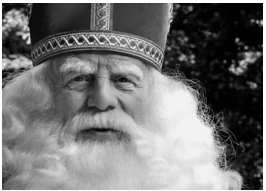
\includegraphics[width=\linewidth]{figures/sint-before.png}
        \caption{Voor \emph{histogram equalization}}
        \label{fig:sinterklaas1}
    \end{minipage}
    \begin{minipage}{0.45\textwidth}
        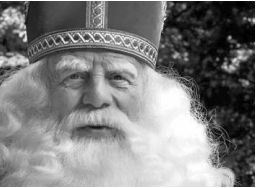
\includegraphics[width=\linewidth]{figures/sint-after.png}
        \caption{Na \emph{histogram equalization}}
        \label{fig:sinterklaas2}
    \end{minipage}
\end{figure}

\subsubsection{Segmentator}

De \emph{segmentator} verzorgt de segmentatie van ontvangen frames. Het hele frame
afgegaan waarbij elke pixel wordt vergeleken met zijn omgeving. De pixel waarden
van de omgeving worden geïntegreerd waarna deze waarde in de pixel wordt gezet
die met zijn omgeving is vergeleken.

\subsubsection{Feature extractor}

Nadat alle pixels zijn geïntegreerd met hun omgeving wordt er gekeken welke Haar
features er aanwezig zijn in het beeld. Dit wordt gedaan door van elke Haar
feature de gemiddelde pixelwaarde van het donkere deel af te trekken van de
gemiddelde pixel waarde van het lichte deel. Als deze waarde boven een bepaalde
threshold ligt wordt er aangenomen dat de Haar feature aanwezig is in de regio
van het beeld waar op dat moment naar wordt gekeken. OpenCV verzorgd standaard
een aantal files die Haar features beschrijven, waaronder één die een gezicht
van de voorkant beschrijft. In het Autonerf systeem wordt dit bestand gebruikt.

\begin{figure}[H]
    \begin{center}
        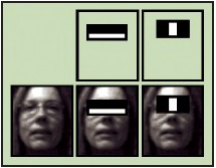
\includegraphics[scale=0.75]{figures/haar-features.png}
        \caption{Haar features in een gezicht}
    \end{center}
\end{figure}

\vfill
\pagebreak

\subsubsection{Classifier}

De door de \emph{feature extractor} beschreven Haar features en thresholds worden
bepaald door een techniek voor \emph{machine-learning} genaamd AdaBoost. Met deze
techniek wordt er per regio gekeken of een door AdaBoost geselecteerde Haar
feature aanwezig is. Als dit niet het geval is wordt de regio direct afgeschreven
als gezicht. Als het wél het geval is gaat de regio door naar de volgende \emph{stage}
en wordt een andere feature geselecteerd, et cetera. Als de regio succesvol alle
\emph{stages} passeert is er sprake van een gezicht.

\begin{figure}[H]
    \begin{center}
        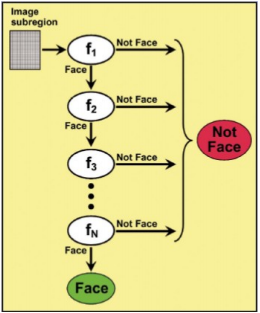
\includegraphics[scale=0.75]{figures/adaboost-classification.png}
        \caption{AdaBoost classificatie}
    \end{center}
\end{figure}

\subsection{De \emph{localizer}}

Het lokaliseren van gezichten is eigenlijk een triviale taak. Zodra de coordinaten
(binnen het frame) bekend zijn van het gezicht, kan hiermee de ruimtelijke
afwijking van het gezicht ten opzichte van het centrum van het frame.

Als we het centrum van het frame $(0, 0)$ dopen, kan de locatie van het gezicht
worden geschreven als $(x, y)$. Een camera heeft een zogenaamd
\emph{field of view} (FOV) wat in graden wordt uitegedrukt. Door middel van deze
eigenschap van de camera, kan precies berekend worden hoeveel graden per pixel
er in het frame zitten (zowel horizontaal als verticaal).

Als voorbeeld nemen we een camera die een resolutie heeft van $640 \times 480$
pixels en een FOV van $45\,^{\circ}$. Hieruit volgt dat het aantal graden per pixel
is: $45\,^{\circ} / 640 = 0.07{\rm \,^{\circ}/p}$ horizontaal en
$45\,^{\circ} / 480 = 0.09{\rm \,^{\circ}/p}$ verticaal. De algemene vergelijking
is te zien in \ref{eq:dpp}. In deze vergelijking is $G_x,_y$ het aantal graden
per pixel in het frame. $F$ is de \emph{field of view} van de camera en $R_x,_y$
is de resolutie van de $x$ en $y$ as.

\begin{equation}
    G_x,_y = \frac{F}{R_x,_y}
    \label{eq:dpp}
\end{equation}

\vfill
\pagebreak

Daarnaast moet er ook een afwijking in pixels worden berekend. Om dit te doen
wordt gebruik gemaakt van het originele frame dat ontvangen is. Door de resolutie
van dit frame te gebruiken (de $R,_y$ uit de vergelijking \ref{eq:dpp}) kan de
afwijking zowel horizontaal als vertikaal worden berekend (vergelijking \ref{eq:offset}).

\begin{equation}
    \Delta_x,_y = {L_x,_y} - {C_x,_y}
    \label{eq:offset}
\end{equation}

In deze vergelijking is $\Delta_x,_y$ de \emph{offset}, $C_x,_y$ is het centrum
van het frame (als een frame $(640,480)$ pixels is, is het
centrum van dit frame $(320,240)$). $L_x,_y$ is de locatie van het gedetecteerde
gezicht wat door de \emph{detector} gedetecteerd is.

Door vergelijking \ref{eq:dpp} en \ref{eq:offset} combineren, is het mogelijk
de offset van het gedetecteerde gezicht in graden uit te drukken (vergelijking
\ref{eq:combined}).

\begin{equation}
    \Delta_x,_y = \frac{F}{R_x,_y}({L_x,_y} - {C_x,_y})
    \label{eq:combined}
\end{equation}

Het is echter voor het systeem niet mogelijk om precies op 0 te komen, daarom
is er een foutmarge geïmplementeerd (de \emph{margin}, $m$). Als $\Delta_x,_y$ binnen
deze \emph{margin} valt, wordt de offset naar 0 gebracht.

\begin{equation}
    \Delta_x,_y = \begin{cases}
        \Delta_x,_y, & \text{als } \Delta_x,_y \geq m\\
        0 & \text{als } \Delta_x,_y < m
    \end{cases}
\end{equation}

Zoals te zien in listing \ref{ls:offset} is dit relatief makkelijk te implementeren
in C++.

\begin{listing}[H]
    \begin{cppcode}
    double dpp[] = {
        ((double) this->fov) / ((double) frame.cols)),
        ((double) this->fov) / ((double) frame.rows))
    };
    int offset[] = {
        (x - (frame.cols / 2)),
        (y - (frame.rows / 2))
    };
    int radial[] = {
        ((double) offset[0]) * dpp[0],
        ((double) offset[1]) * dpp[1]
    };

    if (offset[0] < this->margin &&
        offset[1] < this->margin &&
        offset[0] > -(this->margin) &&
        offset[1] > -(this->margin)) {
        this->emit(
            "fire"
        );
    } else {
        this->emit(
            "localized",
            // Location data
        );
    }
    \end{cppcode}
    \caption{Het \emph{localizen} van gedetecteerde gezichten}
    \label{ls:offset}
\end{listing}

\vfill
\pagebreak

\subsection{De \emph{controller}}

De \emph{controller} is verantwoordelijk voor het aansturen van het Autonerf
systeem. Dit gebeurd middels een seriële verbinding waar JSON-data over verstuurd
wordt. Voor de seriële communicatie wordt gebruik gemaakt van een Boost library
(\code{boost::asio}).

Omdat alle data binnen het systeem ook als JSON wordt verzonden, kunnen de
events van die de \emph{localizer} klasse verstuurd gebruikt worden om het
embedded systeem aan te sturen. Om deze rede heeft de \emph{controller} weinig
logica. Er wordt alleen geschreven naar een seriele port (bijvoorbeeld \code{/dev/tty.usbmodem}).
Hoe dit wordt gedaan wordt getoond in listing \ref{ls:serial}. In deze listing
is de \code{this->serial} variabele een object van de \code{boost::asio::serial\_port}
klasse. De data die verzonden wordt is te zien in listing \ref{ls:output}.

\begin{listing}[H]
    \begin{cppcode}
    void
    Controller::write(const std::string& data)
    {
        boost::asio::write(this->serial, boost::asio::buffer(data.c_str(), data.size()));
    }
    \end{cppcode}
    \caption{Schrijven naar een seriële port}
    \label{ls:serial}
\end{listing}

\begin{listing}[H]
    \begin{jsoncode}
    {"command": "aim", "options": {"offset": [-0.38671875, 3.4375]}}
    {"command": "fire", "options": {}}
    \end{jsoncode}
    \caption{Output over de seriële port}
    \label{ls:output}
\end{listing}
